\chapter{Extremal Kerr black hole}
\label{s:exk}

\minitoc

\section{Introduction}

The Kerr solution of Einstein equation has been introduced in Sec.~\ref{s:ker:Kerr_solution};
it depends on two parameters: the mass $m > 0$ and the spin parameter
$a \geq 0$.
In Chaps.~\ref{s:ker}--\ref{s:gik}, we have considered the Kerr solution with $0<a<m$,
while the case $a=0$ (Schwarzschild solution) has been treated in Chaps.~\ref{s:sch}--\ref{s:max}.
Here we focus on the case $a=m$. As we going to see, it has many properties that are not
shared by the Kerr solution with $a<m$. In particular, the black hole event horizon is
degenerate, in the sense defined in Sec.~\ref{s:neh:classif_KH}: the surface gravity
$\kappa$ vanishes. Note that $a=m$ corresponds to the highest value of $a$
for which the Kerr solution corresponds to a black hole.
Indeed, for $a> m$, the Kerr metric is still an exact
solution of the vacuum Einstein equation, but it describes a \emph{naked singularity}\index{naked singularity} (cf. Sec.~\ref{s:max:naked_sing}):
the ring curvature singularity is not hidden by any black hole horizon to asymptotic observers.


%%%%%%%%%%%%%%%%%%%%%%%%%%%%%%%%%%%%%%%%%%%%%%%%%%%%%%%%%%%%%%%%%%%%%%%%%%%%%%%

\section{Definition and basic properties}

\subsection{The extremal Kerr solution}

Let us consider the manifold $\R^2\times\SS^2$ and describe it by
coordinates $(\ti, r, \th,\tph)$ such that $(\ti,r)$ cover $\R^2$
and $(\th,\tph)$ are standard spherical coordinates on $\SS^2$.
The \defin{extremal Kerr spacetime}\index{extremal!Kerr spacetime}\index{Kerr!extremal -- spacetime}
of mass $m>0$ is defined as the pair $(\M, \w{g})$ where the manifold $\M$ is the following open subset of $\R^2\times\SS^2$:
\be \label{e:exk:def_M}
 \M := \R^2\times\SS^2 \setminus \ring
\ee
with
\be \label{e:exk:def_ring}
    \ring := \left\{ p \in \R^2\times\SS^2,
        \quad r(p) = 0 \ \mbox{and}\ \th(p) = \frac{\pi}{2} \right\} ,
\ee
and the metric $\w{g}$ has the following expression in terms of the coordinates
$(x^{\tilde{\alpha}}) = (\ti, r, \th,\tph)$:
\be \label{e:exk:metric_Kerr_3p1}
    \encadre{
    \begin{array}{ll}
    g_{\tilde{\mu}\tilde{\nu}}\, \D x^{\tilde{\mu}} \, \D x^{\tilde{\nu}}   = &
    \displaystyle - \left( 1 - \frac{2m r}{\rho^2} \right)  \D \ti^2
    + \frac{4m r}{\rho^2} \D\ti\, \D r
    - \frac{4 m^2  r \sin^2\th}{\rho^2} \,  \D \ti\, \D\tph \\[2ex]
    &\displaystyle  + \left( 1 + \frac{2m r}{\rho^2} \right) \D r^2
     - 2 m \left( 1 + \frac{2m r}{\rho^2} \right) \sin^2\th \, \D r\, \D \tph \\[2ex]
    & \displaystyle + \rho^2 \D \th^2
    + \left( r^2 + m^2 + \frac{2 m^3 r \sin^2\th}{\rho^2} \right)
    \sin^2\th \, \D \tph^2 ,
    \end{array}
    }
\ee
with
\be
    \rho^2 := r^2 + m^2\cos^2\th .
\ee
In this context, the coordinates $(x^{\tilde{\alpha}}) = (\ti, r, \th,\tph)$
are called the
\defin{3+1 Kerr coordinates}\index{3+1!Kerr coordinates}\index{Kerr!coordinates!3+1 --}
and we recognize in (\ref{e:exk:metric_Kerr_3p1}) the limit $a\to m$ of
expression (\ref{e:ker:metric_Kerr_3p1}) for the Kerr metric with $a< m$
in the 3+1 Kerr coordinates.

The metric (\ref{e:exk:metric_Kerr_3p1}) is regular
in all $\M$, since the components $g_{\tilde{\alpha}\tilde{\beta}}$ are singular only
for $\rho=0$, i.e. for $r=0$ and $\th=\pi/2$, which defines  the set $\ring$ that has precisely been excluded in
the definition (\ref{e:exk:def_M}) of $\M$. The Kretschmann curvature
invariant\index{Kretschmann scalar! of Kerr metric} $K := R_{\mu\nu\rho\sigma} R^{\mu\nu\rho\sigma}$
is given by Eq.~(\ref{e:ker:Kretschmann}) with $a=m$; it diverges for $\rho\to 0$. Therefore, as
for the Kerr spacetime with $a<m$ (cf. Sec.~\ref{s:ker:singularities}), we shall call $\ring$ the \defin{ring singularity}\index{ring!singularity}\index{singularity!ring --}
of the extremal Kerr spacetime. Note that, formally, it is not part of the spacetime manifold
[cf. Eq.~(\ref{e:exk:def_M})].

Moreover, the Ricci tensor of the metric (\ref{e:exk:metric_Kerr_3p1}) is identically zero in all
$\M$ (see e.g. the notebook~\ref{s:sam:Kerr_extremal}). Hence, we have:
\begin{greybox}
The metric $\w{g}$ of the extremal Kerr spacetime is a solution of Einstein equation\index{Einstein!equation} (\ref{e:fra:Einstein_eq})
in vacuum ($\w{T}=0$) and with a vanishing cosmological constant ($\Lambda=0$).
\end{greybox}

The inverse metric is
\be \label{e:exk:inv_met_3p1}
    g^{\tilde{\alpha}\tilde{\beta}} = \left(
    \begin{array}{cccc}
    - \left( 1 + \frac{2m r}{\rho^2} \right) & \frac{2m r}{\rho^2} & 0 & 0 \\[1ex]
    \frac{2m r}{\rho^2} & \frac{(r-m)^2}{\rho^2} & 0 & \frac{m}{\rho^2} \\[1ex]
    0 & 0 &\frac{1}{\rho^2} & 0 \\[1ex]
    0 & \frac{m}{\rho^2} & 0 & \frac{1}{\rho^2\sin^2\th}
    \end{array}
    \right) .
\ee


\subsection{Boyer-Lindquist coordinates}

For $a<m$, the Kerr manifold $\M$ has been split in three open regions,
$\M_{\rm I}$, $\M_{\rm II}$ and $\M_{\rm III}$,  separated by the two Killing
horizons $\Hor$ and $\Hor_{\rm in}$
[cf. Eqs.~(\ref{e:ker:def_M_Kerr_spacetime}) and (\ref{e:ker:def_M_BL})].
Since $\Hor$ was defined by $r=r_+:=m + \sqrt{m^2 - a^2}$ [Eq.~(\ref{e:ker:def_H})]
and $\Hor_{\rm in}$
by $r=r_-:=m - \sqrt{m^2 - a^2}$ [Eq.~\ref{e:ker:def_H_in})],
we notice that in the $a\to m$ limit
$r_+ = r_- = m$, so that $\Hor$ and $\Hor_{\rm in}$ coincide and the region
$\M_{\rm II}$, which is bounded by $\Hor$ and $\Hor_{\rm in}$, disappears.
Accordingly, we shall split the extremal Kerr manifold $\M$ in two open regions only,
$\M_{\rm I}$ and $\M_{\rm III}$, separated by a single hypersurface $\Hor$:
\be
    \encadre{\M = \M_{\rm I} \cup \Hor \cup \M_{\rm III} },
\ee
with
\begin{subequations}
\begin{align}
    \M_{\rm I} & := \left\{ p \in \M, \quad r(p) > m \right\} \\
    \Hor & := \left\{ p \in \M, \quad r(p) = m \right\} \label{e:exk:def_H}\\
    \M_{\rm III} & := \left\{ p \in \M, \quad r(p) < m \right\} .
\end{align}
\end{subequations}
\begin{remark}
We are using the notation $\M_{\rm III}$ for the ``second'' region
to be consistent with Chaps.~\ref{s:ker}--\ref{s:gik}, more precisely with
the $a\to m$ limit of the results obtained in these chapters.
\end{remark}
The second order polynomial in $r$ introduced in Chap.~\ref{s:ker},
$\Delta=r^2 - 2 m r + a^2 = (r - r_+)(r - r_-)$ reduces to $\Delta = (r - m)^2$
in the limit $a\to m$. Its double root, $r=m$, defines the hypersurface $\Hor$.


In the region $\M_{\rm BL}:= \M \setminus \Hor = \M_{\rm I} \cup \M_{\rm III}$, one may introduce
the \defin{Boyer-Lindquist coordinates}\index{Boyer-Lindquist coordinates}
$(t,r,\th,\ph)$ such that $(r,\th)$ are the same coordinates as in the
3+1 Kerr coordinates, while $t$ and $\ph$ are related to the 3+1 Kerr coordinates
$\ti$, $r$ and $\tph$ by
\begin{subequations}
\label{e:exk:3p1_Kerr_to_BL}
\begin{align}
    t & = \ti +  \frac{2m^2}{r - m} - 2m \ln \left| \frac{r - m}{m} \right|
            \label{e:exk:3p1_Kerr_to_BL_t} \\
    \ph & = \tph + \frac{m}{r - m} . \label{e:exk:3p1_Kerr_to_BL_ph}
\end{align}
\end{subequations}
The differential versions of these relations are
\begin{subequations}
\label{e:exk:dt_dph}
\begin{align}
    \D t & = \D \ti  - \frac{2m r}{(r- m)^2} \, \D r \\
    \D \ph & = \D \tph - \frac{m}{(r - m)^2 } \, \D r .
\end{align}
\end{subequations}
\begin{remark}
The differential relations (\ref{e:exk:dt_dph}) can be obtained immediately
by substituting $a$ by $m$ in relations (\ref{e:ker:Kerr_3p1_BL}). However, to get the integrated
relations (\ref{e:exk:3p1_Kerr_to_BL}) from their $a<m$ analog
(\ref{e:ker:Kerr_3p1_BL_int}), one must perform an expansion in $\veps := \sqrt{m^2 - a^2}/m$,
taking into account that $r_\pm = m(1\pm\veps)$. One then obtains
(\ref{e:exk:3p1_Kerr_to_BL_t})
up to the additive constant $(2\ln 2) m$, while (\ref{e:exk:3p1_Kerr_to_BL_ph}) is recovered in the same form.
\end{remark}
It follows from the transformations (\ref{e:exk:3p1_Kerr_to_BL}) that
the Boyer-Lindquist coordinate frame $(\wpar_\alpha)$ and the 3+1 Kerr coordinate frame $(\wpar_{\tilde{\alpha}})$ are related by\footnote{See also the $a\to m$ limit of Eq.~(\ref{e:ker:frame_Kerr3p1_BL}).}
\begin{subequations}
\label{e:exk:frame_BL_Kerr3p1}
\begin{align}
    & \wpar_t  = \wpar_\ti  \\
    & \wpar_r = \wpar_{\tilde r} + \frac{2mr}{(r-m)^2} \wpar_\ti
                        + \frac{m}{(r-m)^2} \wpar_\tph \\
    & \wpar_\th = \wpar_\th \\
    & \wpar_\ph = \wpar_{\tph} .
\end{align}
\end{subequations}
Note that, as in Chap.~\ref{s:ker}, we have denoted by $\wpar_{\tilde r}$ the second vector of the
coordinate frame associated to the 3+1 Kerr coordinates
$(x^{\tilde{\alpha}}) = (\ti, r, \th,\tph)$, in order to distinguish it from
the coordinate vector
$\wpar_r$ of the Boyer-Lindquist coordinates
$(x^\alpha) = (t,r,\th,\ph)$.

\begin{figure}
\centerline{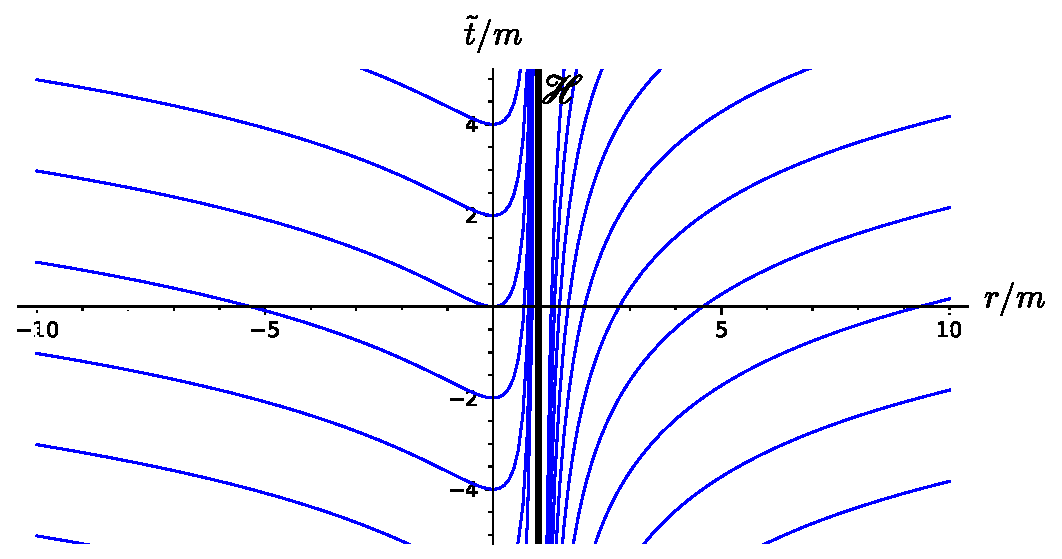
\includegraphics[width=0.7\textwidth]{exk_BL_slicing.pdf}}
\caption[]{\label{f:exk:BL_slicing} \footnotesize
Trace of the hypersurfaces of constant Boyer-Lindquist time $t$ in the plane
$(\tilde{t}, r)$.
\textsl{[Figure generated by the notebook \ref{s:sam:Kerr_extremal}]}
}
\end{figure}

The metric components $(g_{\alpha\beta})$ with respect to the Boyer-Lindquist coordinates $(x^\alpha) = (t,r,\th,\ph)$ are given by
\be \label{e:exk:metric_BL}
    \encadre{
    \begin{array}{ll}
    g_{\mu\nu}\,  \D x^\mu \D x^\nu  = &
    \displaystyle - \left( 1 - \frac{2m r}{\rho^2} \right) \, \D t^2
    - \frac{4 m^2  r \sin^2\th}{\rho^2} \,  \D t\, \D\ph
    + \frac{\rho^2}{(r-m)^2} \, \D r^2  \\[2ex]
    & \displaystyle + \rho^2 \D \th^2
    + \left( r^2 + m^2 + \frac{2 m^3 r \sin^2\th}{\rho^2} \right)
    \sin^2\th \, \D \ph^2 .
    \end{array}
    }
\ee
This expression can be obtained either by taking the limit $a\to m$ of Eq.~(\ref{e:ker:metric_BL})
of by using (\ref{e:exk:dt_dph}) to substitute $\D\ti$ and $\D\tph$ in Eq.~(\ref{e:exk:metric_Kerr_3p1}).
We note that $g_{rr}\to +\infty$ when $r\to m$, which reflects the singularity of Boyer-Lindquist
coordinates on $\Hor$. This singularity is clearly apparent in the coordinate transformations
(\ref{e:exk:3p1_Kerr_to_BL}), as well as in the spacetime slicing by the
hypersurfaces $t=\mathrm{const}$ depicted in Fig.~\ref{f:exk:BL_slicing}: the slices accumulate
onto $\Hor$, without crossing it, so that the points on $\Hor$ do not belong to any
hypersurface $t=\mathrm{const}$.

The inverse metric $\w{g}^{-1}$ has the following components in the Boyer-Lindquist coordinates
(cf. the $a\to m$ limit of Eq.~(\ref{e:ker:inv_met_BL})):
\be \label{e:exk:inv_met_BL}
    g^{\alpha\beta} = \left(
    \begin{array}{cccc}
    - \frac{1}{(r-m)^2}
    \left( r^2 + m^2 + \frac{2 m^3 r \sin^2\th}{\rho^2} \right)
     & 0 & 0 & -\frac{2 m^2 r}{\rho^2 (r-m)^2} \\[1ex]
    0 & \frac{(r-m)^2}{\rho^2} & 0 & 0 \\[1ex]
    0 & 0 &\frac{1}{\rho^2} & 0 \\[1ex]
    -\frac{2 m^2 r}{\rho^2 (r-m)^2} & 0 & 0 &
    \frac{1}{(r-m)^2\sin^2\th}\left(1 - \frac{2 m r}{\rho^2} \right)
    \end{array}
    \right) .
\ee

\subsection{Symetries}

The extremal Kerr metric (\ref{e:exk:metric_Kerr_3p1}) is stationary\footnote{Cf.
Sec.~\ref{s:sta:def_station} for the definition of \emph{stationary} and a discussion
about the terminology.} and axisymmetric. The corresponding isometry group is $\R\times\mathrm{SO}(2)$ and is generated
by two commuting Killing vectors $\w{\xi}$ and $\w{\eta}$. Both the 3+1 Kerr coordinates and
the Boyer-Lindquist ones are adapted to the spacetime symmetries, i.e. $(\ti,\tph)$ and
$(t,\ph)$ are ignorable coordinates, as it is clear on the line elements (\ref{e:exk:metric_Kerr_3p1})
and (\ref{e:exk:metric_BL}). Accordingly, one can normalize the Killing vectors so that
\be
    \encadre{\w{\xi} = \wpar_{\ti} = \wpar_t}
    \qand
    \encadre{\w{\eta} = \wpar_{\tph} = \wpar_\ph} .
\ee

\begin{figure}
\centerline{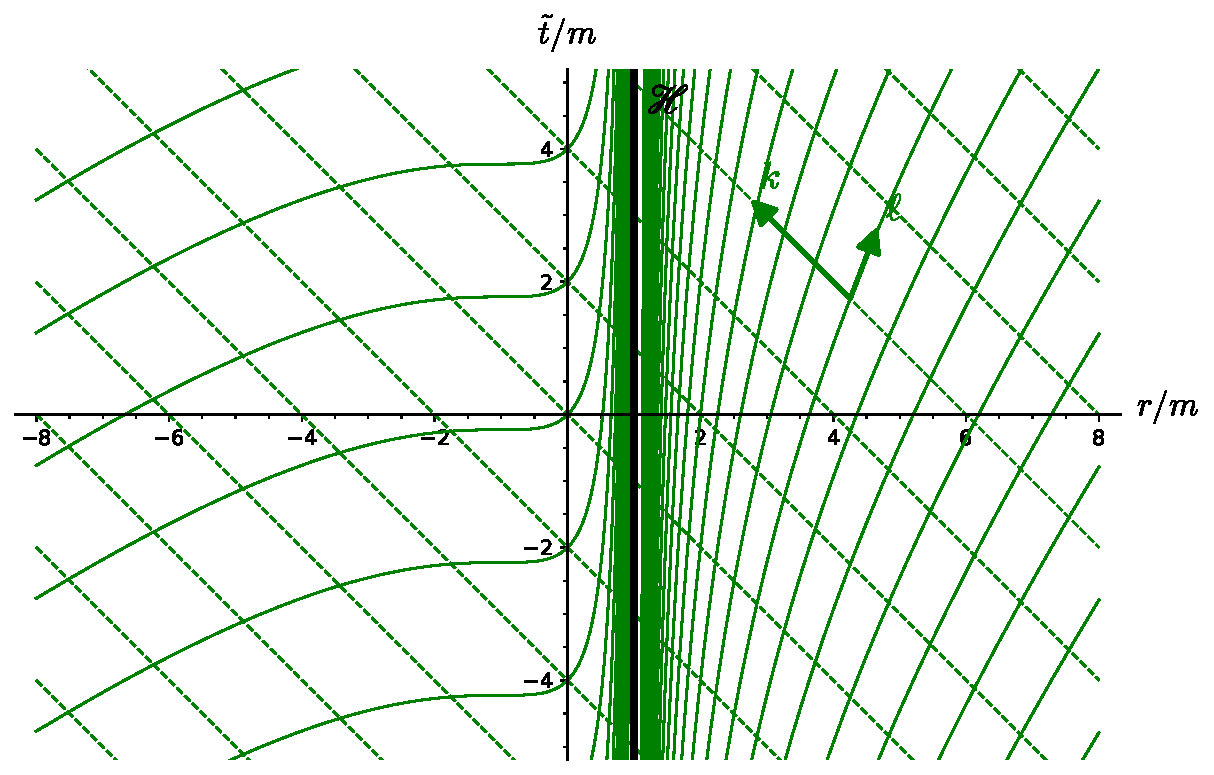
\includegraphics[width=0.8\textwidth]{exk_princ_null_geod.pdf}}
\caption[]{\label{f:exk:princ_null_geod} \footnotesize
Trace of the principal null geodesics in the plane
$(\tilde{t}, r)$. The dashed lines correspond to the
ingoing principal null geodesics $\Li^{\rm in}_{(v,\th,\tph)}$
and the solid curves to the
outgoing principal null geodesics $\Li^{\rm out,I}_{(u,\th,\tilde{\tph})}$
for $r>m$ and $\Li^{\rm out,III}_{(u,\th,\tilde{\tph})}$ for $r<m$.
\textsl{[Figure generated by the notebook \ref{s:sam:Kerr_extremal}]}
}
\end{figure}



\subsection{Principal null geodesics}

As discussed in Sec.~\ref{s:ker:principal_geod}, the Kerr spacetime is
endowed with two congruences of null geodesics that are tied to
the spacetime structure, as described by the Weyl conformal curvature tensor.
All the results of Sec.~\ref{s:ker:principal_geod} remain valid at the limit $a\to m$.
We can summarize them as follows:
\begin{greybox}
\begin{itemize}
\item The \defin{ingoing principal null geodesics} are the curves
\be
    \Li^{\rm in}_{(v,\th,\tph)}: \quad v = \mathrm{const},\ \th=\mathrm{const},\
        \tph=\mathrm{const},
\ee
where $v$ is the Kerr advanced time:
\be \label{e:exk:def_v}
    v := \ti + r = t  + r - \frac{2m^2}{r -m} + 2m\ln\left| \frac{r - m}{m} \right|.
\ee
Along $\Li^{\rm in}_{(v,\th,\tph)}$, $-r$ is an affine parameter increasing towards the future;
the corresponding tangent vector is
\begin{subequations}
\begin{align}
 \w{k} & = \wpar_{\ti} - \wpar_{\tilde{r}} \label{e:exk:k_3p1_Kerr}\\
 \w{k} & = \frac{r^2 + m^2}{(r - m)^2}  \wpar_t
            - \wpar_r + \frac{m}{(r - m)^2} \, \wpar_\ph
            \quad \mbox{in}\ \M\setminus\Hor .  \label{e:exk:k_BL}
\end{align}
\end{subequations}
\item The \defin{outgoing principal null geodesics} are the curves
\begin{subequations}
\begin{align}
  \mbox{in}\ \M_{\rm I} :&\quad \Li^{\rm out, I}_{(u,\th,\tilde{\tph})}:
  \quad u = \mathrm{const},\ \th=\mathrm{const},\
        \tilde{\tph}=\mathrm{const}, \\
  \mbox{in}\ \M_{\rm III}:&\quad \Li^{\rm out, III}_{(u,\th,\tilde{\tph})}:
  \quad u = \mathrm{const},\ \th=\mathrm{const},\
        \tilde{\tph}=\mathrm{const}, \\
 \mbox{on}\  \Hor: &\quad \Li^{{\rm out},\Hor}_{(\th,\psi)}:
    \quad  \th=\mathrm{const},\ \psi = \mathrm{const},
\end{align}
\end{subequations}
where $u$ is the Kerr retarded time:
\be \label{e:exk:def_u}
    u := \ti - r + \frac{4 m^2}{r - m} - 4 m \ln \left| \frac{r - m}{m} \right|
      = t  - r + \frac{2m^2}{r -m} - 2m\ln\left| \frac{r - m}{m} \right| ,
\ee
\be \label{e:exk:def_ttph}
    \tilde{\tph} := \tph + \frac{2m}{r -m} = \ph + \frac{m}{r - m}
\ee
and
\be \label{e:exk:psi_tph_ti}
    \psi := \tph - \frac{\ti}{2m} .
\ee
Along $\Li^{\rm out, I}_{(u,\th,\tilde{\tph})}$ and $\Li^{\rm out, III}_{(u,\th,\tilde{\tph})}$,
$r$ is an affine parameter increasing towards the future,
while along $\Li^{{\rm out},\Hor}_{(\th,\psi)}$, such an affine parameter is $\ti$. The null tangent vector $\wl$ along the outgoing principal null geodesics
that coincides with the Killing vector $\w{\xi} + (2m)^{-1} \w{\eta}$ on $\Hor$ is
\begin{subequations}
\begin{align}
 \wl & = \left( \frac{1}{2}  + \frac{m r}{r^2 + m^2}\right) \wpar_{\ti}
  +  \left( \frac{1}{2} - \frac{m r}{r^2 + m^2}\right) \wpar_{\tilde{r}}
  + \frac{m}{r^2 + m^2} \wpar_{\tph} \label{e:exk:ell_3p1_Kerr}\\
 \wl & =  \frac{1}{2} \wpar_t
            + \left( \frac{1}{2}  - \frac{m r}{r^2 + m^2} \right) \wpar_r
            + \frac{m}{2(r^2 + m^2)} \, \wpar_\ph
            \quad \mbox{in}\ \M\setminus\Hor . \label{e:exk:ell_BL}
\end{align}
\end{subequations}
\end{itemize}
\end{greybox}
\begin{proof}
The second equality in Eq.~(\ref{e:exk:def_v}) follows from Eq.~(\ref{e:exk:3p1_Kerr_to_BL_t}).
Eq.~(\ref{e:exk:k_BL}) follow from Eq.~(\ref{e:exk:k_3p1_Kerr}) via Eq.~(\ref{e:exk:frame_BL_Kerr3p1}).
Eqs.~(\ref{e:exk:def_u}) and (\ref{e:exk:def_ttph}) are the integrated version of the system (\ref{e:ker:out_Kerr_Kerr_3p1}) with $a=m$. Equations~(\ref{e:exk:psi_tph_ti}), (\ref{e:exk:ell_3p1_Kerr})
and (\ref{e:exk:ell_BL}) are the $a=m$ versions of respectively
Eqs.~(\ref{e:ker:psi_tph_ti}), (\ref{e:ker:def_ell_outgoing}) and (\ref{e:ker:ell_BL}).
All the other statements follow from the $a\to m$ limit of results of Sec.~\ref{s:ker:principal_geod},
except for $\ti$ being an affine parameter along $\Li^{{\rm out},\Hor}_{(\th,\psi)}$, which
is peculiar to the extremal Kerr horizon and will
be proved in Sec.~\ref{s:exk:horizon}.
\end{proof}

The principal null geodesic congruences are depicted in terms of the $(\ti, r)$
coordinates in Fig.~\ref{f:exk:princ_null_geod}.


\subsection{The degenerate horizon} \label{s:exk:horizon}

$\Hor$ is the hypersurface of $\M$ defined by $r=m$ [Eq.~(\ref{e:exk:def_H})]. Given
that the component $g^{rr} = (r - m)^2/\rho^2$ of the inverse metric with respect to 3+1 Kerr coordinates vanishes at $r=m$ [cf. Eq.~(\ref{e:exk:inv_met_3p1})], we have
$g^{\tilde{\mu}\tilde{\nu}} \partial_{\tilde{\mu}} r \partial_{\tilde{\nu}} r = 0$ on $\Hor$,
which implies that the gradient $\vw{\nabla} r$
is a null vector there and that $\Hor$ is a null hypersurface.
Moreover, since the components of $\vw{\nabla} r$ are $\nabla^{\tilde{\alpha}} = g^{\tilde{\alpha}r}$,
we read on Eq.~(\ref{e:exk:inv_met_3p1}) that
\be
    \vw{\nabla} r \equalH \frac{2m^2}{\rho^2} \wpar_{\ti} + \frac{m}{\rho^2} \wpar_{\tph}
        \equalH \frac{2 m^2}{\rho^2} \w{\chi} ,
\ee
where $\w{\chi}$ is the Killing vector field
\be
    \w{\chi} := \w{\xi} + \Omega_H \w{\eta} , \qquad\mbox{with}\quad \Omega_H := \frac{1}{2m} .
\ee
It follows immediately that $\Hor$ is a \emph{Killing horizon}, i.e. a null hypersurface
that admits a Killing vector as null normal (cf. the definition given in
Sec.~\ref{s:neh:def_Killing_hor}).

From expression~(\ref{e:exk:ell_3p1_Kerr}) for $\wl$, we have immediately
\be \label{e:exk:ell_chi_on_H}
    \wl \equalH \w{\chi} .
\ee
This means that the null generators of $\Hor$ are the outgoing principal null
geodesics $\Li^{{\rm out},\Hor}_{(\th,\psi)}$.

The \emph{surface gravity}\index{surface!gravity} $\kappa$ of the Killing horizon $\Hor$
has been defined in Sec.~\ref{s:neh:zeroth_law} as the non-affinity coefficient of the Killing-vector normal $\w{\chi}$ to $\Hor$:
$\wnab_{\w{\chi}}\, \w{\chi} \equalH \kappa \, \w{\chi}$ [cf. Eq.~(\ref{e:neh:xi_nab_xi_kappa})].
Given (\ref{e:exk:ell_chi_on_H}), $\kappa$ coincides with the value on $\Hor$ of the
non-affinity coefficient $\kappa_{\wl}$ of the tangent $\wl$ to the outgoing principal null
geodesics: $\wnab_{\wl}\, \wl = \kappa_{\wl}\, \wl$. A direct computation (cf. the notebook~\ref{s:sam:Kerr_extremal}) reveals that
\be
    \kappa_{\wl} = m \frac{r^2 - m^2}{(r^2 + m^2)^2} .
\ee
In particular, $\kappa_{\wl}$ vanishes for $r=m$, i.e. on $\Hor$.
Since $\kappa = \left. \kappa_{\wl} \right| _{\Hor}$, we
get\footnote{The vanishing of $\kappa$ can also be obtained
by taking the limit $a\to m$ of expression (\ref{e:ker:kappa_m_a}) derived for $a<m$.}
\be
    \encadre{\kappa = 0 } .
\ee
According to the classification introduced in Sec.~\ref{s:neh:classif_KH}, one says
that $\Hor$ is a \emph{degenerate Killing horizon}\index{degenerate!Killing horizon}\index{Killing!horizon!degenerate --}.


\section{Maximal analytic extension}

\section{Near-horizon extremal Kerr metric}

\subsection{The extremal Kerr throat}


